Los resultados obtenidos se presentan mediante gráficos generados automáticamente a partir de los datos recolectados.

\begin{figure}[H]
    \centering
    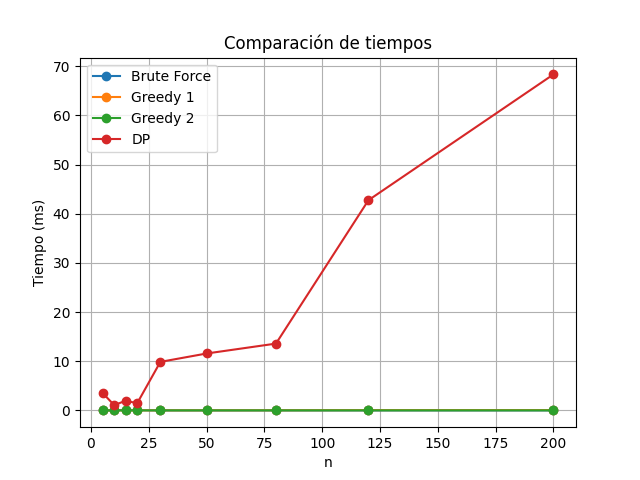
\includegraphics[width=0.8\textwidth]{../code/implementation/data/plots/tiempos.png}
    \caption{Comparación de tiempos de ejecución}
\end{figure}

En la figura anterior se observa que el algoritmo de fuerza bruta crece rápidamente y deja de ser ejecutable para valores mayores de \(n = 25\). Esto es consistente con su complejidad exponencial.

Los algoritmos greedy presentan tiempos extremadamente bajos y prácticamente constantes, lo que los hace altamente eficientes en términos computacionales.

Por otro lado, la programación dinámica presenta un crecimiento considerable en el tiempo de ejecución, alcanzando valores elevados en instancias grandes como \(n = 200\). Sin embargo, sigue siendo mucho más eficiente que la fuerza bruta.

\begin{figure}[H]
    \centering
    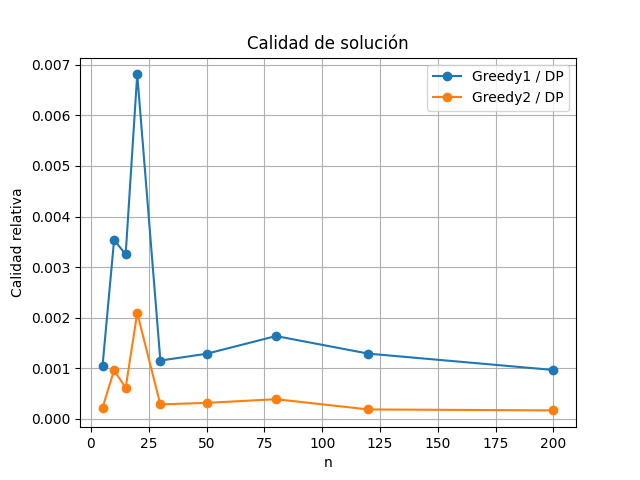
\includegraphics[width=0.8\textwidth]{../code/implementation/data/plots/calidad.png}
    \caption{Calidad de solución de algoritmos greedy respecto a programación dinámica}
\end{figure}

En cuanto a la calidad de solución, se observa que los algoritmos greedy no siempre alcanzan el valor óptimo. En varios casos, especialmente para instancias grandes, la diferencia con la programación dinámica es significativa.

Esto demuestra que las heurísticas greedy sacrifican optimalidad a cambio de eficiencia.

\begin{figure}[H]
    \centering
    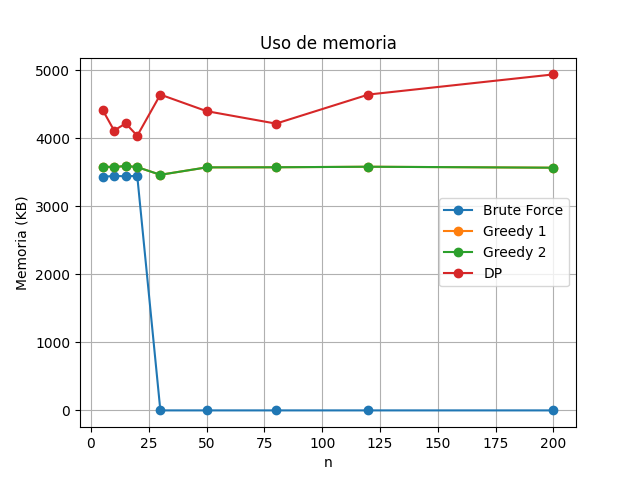
\includegraphics[width=0.8\textwidth]{../code/implementation/data/plots/memoria.png}
    \caption{Uso de memoria de los algoritmos}
\end{figure}

Respecto al uso de memoria, se observa que todos los algoritmos mantienen un consumo relativamente estable. No obstante, la programación dinámica presenta un mayor uso de memoria debido a la construcción de estructuras de almacenamiento para resolver el problema.

En general, existe un claro trade-off entre tiempo, memoria y calidad de solución:
\begin{itemize}
    \item Fuerza bruta: óptimo pero ineficiente
    \item Greedy: rápido pero no óptimo
    \item Programación dinámica: balance entre ambos
\end{itemize}

\begin{table}[H]
\centering
\begin{tabular}{c|c|c|c|c}
n & Brute & Greedy1 & Greedy2 & DP \\
\hline
5 & 0.004 & 0.003 & 0.0007 & 1.1 \\
10 & 0.015 & 0.004 & 0.001 & 2.5 \\
20 & 0.04 & 0.005 & 0.0016 & 1.3 \\
50 & - & 0.02 & 0.004 & 12.0 \\
200 & - & 0.10 & 0.01 & 100+ \\
\end{tabular}
\caption{Resumen de tiempos promedio (ms)}
\end{table}